\documentclass{article}%
\usepackage{amsmath}
\usepackage{amsfonts}
\usepackage{amssymb}
\usepackage{graphicx}
\usepackage{tikz}
\usepackage{hyperref}%
\setcounter{MaxMatrixCols}{30}
%TCIDATA{OutputFilter=latex2.dll}
%TCIDATA{Version=5.00.0.2552}
%TCIDATA{CSTFile=40 LaTeX article.cst}
%TCIDATA{Created=Thursday, August 21, 2008 14:03:59}
%TCIDATA{LastRevised=Wednesday, October 01, 2014 12:46:33}
%TCIDATA{<META NAME="GraphicsSave" CONTENT="32">}
%TCIDATA{<META NAME="SaveForMode" CONTENT="1">}
%TCIDATA{<META NAME="DocumentShell" CONTENT="Standard LaTeX\Blank - Standard LaTeX Article">}
%TCIDATA{Language=American English}
\newtheorem{theorem}{Theorem}
\newtheorem{acknowledgement}[theorem]{Acknowledgement}
\newtheorem{algorithm}[theorem]{Algorithm}
\newtheorem{axiom}[theorem]{Axiom}
\newtheorem{case}[theorem]{Case}
\newtheorem{claim}[theorem]{Claim}
\newtheorem{conclusion}[theorem]{Conclusion}
\newtheorem{condition}[theorem]{Condition}
\newtheorem{conjecture}[theorem]{Conjecture}
\newtheorem{corollary}[theorem]{Corollary}
\newtheorem{criterion}[theorem]{Criterion}
\newtheorem{definition}[theorem]{Definition}
\newtheorem{example}[theorem]{Example}
\newtheorem{exercise}[theorem]{Exercise}
\newtheorem{lemma}[theorem]{Lemma}
\newtheorem{notation}[theorem]{Notation}
\newtheorem{problem}[theorem]{Problem}
\newtheorem{proposition}[theorem]{Proposition}
\newtheorem{remark}[theorem]{Remark}
\newtheorem{solution}[theorem]{Solution}
\newtheorem{summary}[theorem]{Summary}
\newenvironment{proof}[1][Proof]{\noindent\textbf{#1.} }{\ \rule{0.5em}{0.5em}}
\begin{document}

\title{Homework 2}
\author{Christopher Chapline}
\maketitle

\section{Exercise 2.3.2}
\begin{center}
    \begin{tabular}{a b|c|d}
        & 0 & 1 \\ \hline
        start\rightarrow & $\{p\}$ & $\{q, s\}$ & $\{q\}$ \\ \hline
          & $\{r\}$ & $\{s\}$ & $\{p\}$ \\ \hline
        * & $*\{s\}$ & $\emptyset$ & $\{p\}$ \\ \hline
        * & $*\{q\}$ & $\{r\}$ & $\{q, r\}$ \\ \hline
        * & $*\{q, r\}$ & $\{q, s\}$ & $\{q, r, p\}$ \\ \hline
        * & $*\{q, s\}$ & $\{r\}$ & $\{q, r, p\}$ \\ \hline
        & $\emptyset$ & $\emptyset$ & $\emptyset$ \\ \hline
        * & $*\{q, r, p\}$ & $\{r, s, q\}$ & $\{q, r, p\}$ \\ \hline
        * & $*\{r, s, q\}$ & $\{s, r\}$ & $\{q, r, p\}$ \\ \hline
        * & $*\{s, r\}$ & $\{s\}$ & $\{p\}$ \\ \hline
    \end{tabular}
\end{center}

\section{Exercise 2.3.3}

This DFA accepts the language containing strings of 0's and 1's that end in one of the following: 00, 01, 001.

\begin{center}
    \begin{tabular}{a b|c|d}
        & 0 & 1 \\ \hline
        start\rightarrow & $\{p\}$ & $\{p, q\}$ & $\{p\}$ \\ \hline
        & $\{q\} & $\{r, s\}$ & $\{t\}$ \\ \hline
        & $\{r\} & $\{p, r\}$ & $\{t\}$ \\ \hline
        * & $\{s\}$ & $\emptyset$ & $\emptyset$ \\ \hline
        * & $\{t\}$ & $\emptyset$ & $\emptyset$ \\ \hline
        & $\{p, q\}$ & $\{p, q, r, s\}$ & $\{p\}$ \\ \hline
        * & $\{r, s\}$ & $\{p, q\}$ & $\{t\}$ \\ \hline
          & $\{p, r\}$ & $\{p, q, r\}$ & $\{p, t\}$ \\ \hline
        & $\emptyset$ & $\emptyset$ & $\emptyset$ \\ \hline
        * & $\{p, q, r, s\}$ & $\{p, q, r\}$ & $\{p, t\}$ \\ \hline
        & $\{p, q, r\}$ & $\{p, q\}$ & $\{p, t\}$ \\ \hline
        * & $\{p, t\}$ & $\{p, q\}$ & $\{p\}$ \\ \hline
    \end{tabular}
\end{center}

\section{Exercise 2.3.4(a)}

\begin{center}
    \begin{tabular}{s|z|o|e|n} %prefix state | zero | one | elipses | nine
        & 0 & 1 & ... & 9 \\ \hline
        \rightarrow s & $a_0 \cup \{w_0, ..., w_9\} \cap w_0$ & $a_1 \cup \{w_0, ..., w_9\} \cap w_1$ & ... & $a_9 \cup \{w_0, ..., w_9\} \cap w_9$ \\ \hline
        *$a_0$ & \emptyset & \emptyset & ... & \emptyset \\ \hline
        $w_0$ & $a_0$ & $w_0$ & ... & $w_0$ \\ \hline
        *$a_1$ & \emptyset & \emptyset & ... & \emptyset \\ \hline
        $w_1$ & $w_1$ & $a_1$ & ... & $w_1$ \\ \hline
        ... & ... & ... & ... & ... \\ \hline
        *$a_9$ & \emptyset & \emptyset & ... & \emptyset \\ \hline
        $w_9$ & $w_9$ & $w_9$ & ... & $a_9$ \\ \hline
    \end{tabular}
\end{center}


In this NFA, the states labeled $a_i$ are accepting states for the symbol $i$. The states labeled $w_i$ are "waiting states" for the symbol $i$. Waiting states will transition to themselves on all input
that is not $i$ and when $i$ is encountered, they transition to $a_i$. In the start state, this NFA will transfer to nine waiting states and one accepting state upon reading the first symbol $j$. These states
will be $a_j \cup \{w_0, ..., w_9\} \cap w_j$.


\section{Exercise 2.3.4(b)}

\begin{center}
    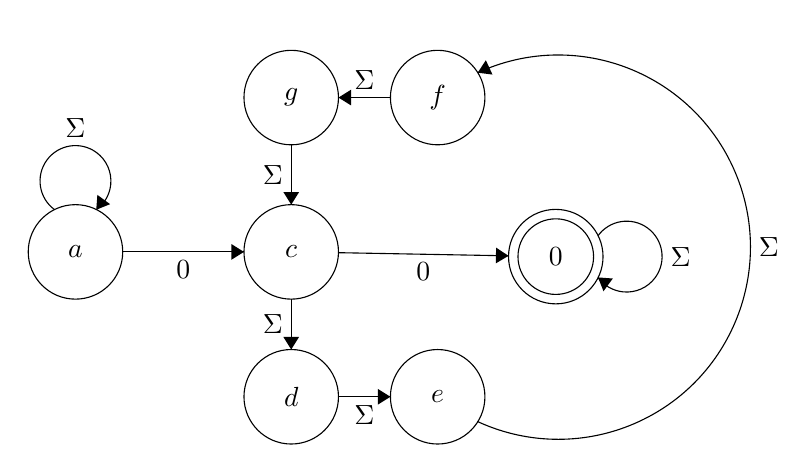
\begin{tikzpicture}[scale=0.2]
        \tikzstyle{every node}+=[inner sep=0pt]
        \draw [black] (6.7,-28.9) circle (3);
        \draw (6.7,-28.9) node {$a$};
        \draw [black] (20.4,-28.9) circle (3);
        \draw (20.4,-28.9) node {$c$};
        \draw [black] (20.4,-38.1) circle (3);
        \draw (20.4,-38.1) node {$d$};
        \draw [black] (29.7,-38.1) circle (3);
        \draw (29.7,-38.1) node {$e$};
        \draw [black] (20.4,-19.1) circle (3);
        \draw (20.4,-19.1) node {$g$};
        \draw [black] (29.7,-19.1) circle (3);
        \draw (29.7,-19.1) node {$f$};
        \draw [black] (37.2,-29.2) circle (3);
        \draw (37.2,-29.2) node {$0$};
        \draw [black] (37.2,-29.2) circle (2.4);
        \draw [black] (20.4,-31.9) -- (20.4,-35.1);
        \fill [black] (20.4,-35.1) -- (20.9,-34.3) -- (19.9,-34.3);
        \draw (19.9,-33.5) node [left] {$\Sigma$};
        \draw [black] (23.4,-38.1) -- (26.7,-38.1);
        \fill [black] (26.7,-38.1) -- (25.9,-37.6) -- (25.9,-38.6);
        \draw (25.05,-38.6) node [below] {$\Sigma$};
        \draw [black] (32.243,-17.522) arc (114.78329:-114.78329:12.202);
        \fill [black] (32.24,-17.52) -- (33.18,-17.64) -- (32.76,-16.73);
        \draw (50.06,-28.6) node [right] {$\Sigma$};
        \draw [black] (26.7,-19.1) -- (23.4,-19.1);
        \fill [black] (23.4,-19.1) -- (24.2,-19.6) -- (24.2,-18.6);
        \draw (25.05,-18.6) node [above] {$\Sigma$};
        \draw [black] (5.377,-26.22) arc (234:-54:2.25);
        \draw (6.7,-21.65) node [above] {$\Sigma$};
        \fill [black] (8.02,-26.22) -- (8.9,-25.87) -- (8.09,-25.28);
        \draw [black] (20.4,-22.1) -- (20.4,-25.9);
        \fill [black] (20.4,-25.9) -- (20.9,-25.1) -- (19.9,-25.1);
        \draw (19.9,-24) node [left] {$\Sigma$};
        \draw [black] (9.7,-28.9) -- (17.4,-28.9);
        \fill [black] (17.4,-28.9) -- (16.6,-28.4) -- (16.6,-29.4);
        \draw (13.55,-29.4) node [below] {$0$};
        \draw [black] (23.4,-28.95) -- (34.2,-29.15);
        \fill [black] (34.2,-29.15) -- (33.41,-28.63) -- (33.39,-29.63);
        \draw (28.79,-29.57) node [below] {$0$};
        \draw [black] (39.88,-27.877) arc (144:-144:2.25);
        \draw (44.45,-29.2) node [right] {$\Sigma$};
        \fill [black] (39.88,-30.52) -- (40.23,-31.4) -- (40.82,-30.59);
    \end{tikzpicture}
\end{center}

\end{document}
